%% Packages indispensables
\documentclass[a4paper, 12pt]{article}
\usepackage[utf8]{inputenc}
\usepackage[T1]{fontenc}
\usepackage[english]{babel}

\usepackage[a4paper]{geometry}
\usepackage{graphicx}

\newcommand{\package}[1]{\texttt{#1}}
\newcommand{\kv}[2]{\textit{<#1>}\texttt=\textit{<#2>}}
\newcommand{\key}[3]{\textbf{\texttt{#1} (default value: \texttt{#2})} #3}
\newcommand{\commande}[1]{\texttt{\textbackslash#1}}


\usepackage{hyperref}
\hypersetup{
	colorlinks=true,
	linkcolor=blue,
	urlcolor=blue,
}

\title{Package \texttt{playcards.sty} for \LaTeX}
\date{\today}
\author{Clément Pagès \texttt{contact -- arobase -- clementpages point fr}}

\begin{document}
\maketitle

This small package provides commands to draw playcards, with witdh 59 mm and height 89 mm, which are typicall cards dimensions.

\tableofcontents
\section*{Thanks}
Thanks to Christophe Poulain for his amazing \href{https://ctan.org/pkg/profcollege}{ProfCollege} package, which source code was useful to design syntax commands we use here. And more generally, thank you you for this amazing package!

Also thanks to \href{https://tex.stackexchange.com/users/1948/didest}{didest} who asked a question on \href{https://tex.stackexchange.com/questions/47924/creating-playing-cards-using-tikz}{StackExchange}. I used it to built this package.

\section{Download, installation, requirements}

Package available on CTAN. It contains one single file : \texttt{playcards.sty}.

Some package are automatically loaded. They are installed by default on most configurations :
\begin{description}
	\item[\package{tikz}] and some libraries.
	\item[\package{simplekv}] dot manage optional parameters whit a \kv{key}{value} system.
	\item[\package{graphicx}] for pictures. 
	\item[\package{contour}] for text shadows and borders.
	\item[\package{geometry}] configured to draw 9 cards on an A4 paper.
\end{description}

\section{Generalities}
Commands are based on a key/value system, with model \texttt{\textbackslash command[\kv{key1}{value1}, \kv{key2}{value2}, …,]\{param1\}\{param2\}}.

All the keys are optional and if one does not fill them, they get a default value.

All length are given in millimeters.

\section{Provided commands}
	\subsection{\commande{drawcardsrecto} command}
This command has one required parameter : text written in the center of the card. It fills an A4 paper with 9 identical cards. This command only draws front side of the card. There is an example figure \ref{fig:recto}.
\begin{figure}[h]\begin{center}
	\caption{\commande{drawcardsrecto[trame=false]\{5\}}}
	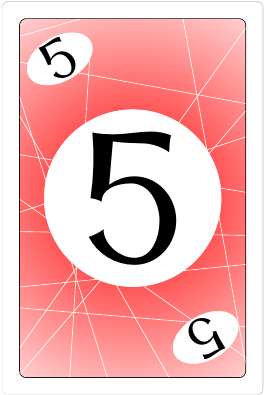
\includegraphics{screen01.png}\label{fig:recto}
\end{center}\end{figure}

Optional parameters:
\begin{itemize}
	\item \key{borders}{true}{Removes borders.}
	\item \key{trame}{true}{If \texttt{true}, fills an A4 paper with cards.. Si \texttt{false}, draws one only card.}
	\item \key{corners}{true}{If \texttt{true}, card contends is reproduced in corners. If \texttt{false}, it is not.}
	\item \key{backgroundImg}{true}{Si \texttt{true}, prints background. If \texttt{false}, no background.}
	\item \key{backgroundColor}{red}{Specifies background color. Ignored if \texttt{backgroundImg=false}. Uses colored defined in the \href{https://www.ctan.org/pkg/xcolor}{xcolor} package.}
	\item \key{contentsFontSize}{120}{Font size (int pt) of text in card center.}
	\item \key{cicleRay}{20}{Ray of the white circle the center of the card. Value \texttt 0 means no circle.}
\end{itemize}


	\subsection{\commande{drawcardsverso} command}
It is possible, but not required, to draw card back side. Front sides must be on one page and back sides on an other. You must have as many front sides as back sides. There is an example figure \ref{fig:verso}.

To get a correct alignment, place commands in a  \verb!\begin{center}...\end{center}! environment.
\begin{figure}[h]\begin{center}
	\caption{\commande{drawcardsverso[trame=false,contentsFontSize=40]\{Exemple\}}}
	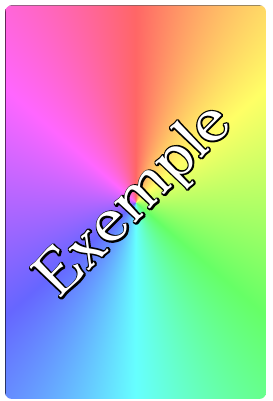
\includegraphics{screen02.png}\label{fig:verso}
\end{center}\end{figure}

Optional parameters:
\begin{itemize}
	\item \key{backgroundImg}{true}{Si \texttt{true}, prints background. If \texttt{false}, no background.}
	\item \key{trame}{true}{If \texttt{true}, fills an A4 paper with cards.. Si \texttt{false}, draws one only card.}
	\item \key{contentsFontSize}{120}{Font size (int pt) of text in card center.}
\end{itemize}

\end{document}
